\subsection{UNet+++}
We test the relationship between epoch and the accuracy of test data, in order to find the best epoch value. In the test, the value of epoch range from 1 to 40. 
In each iteration, we test the current model on test dataset, and record the accuracy. The result is given Figure.\ref{fig:unetpppCurve}.

\begin{figure}[!htpb]
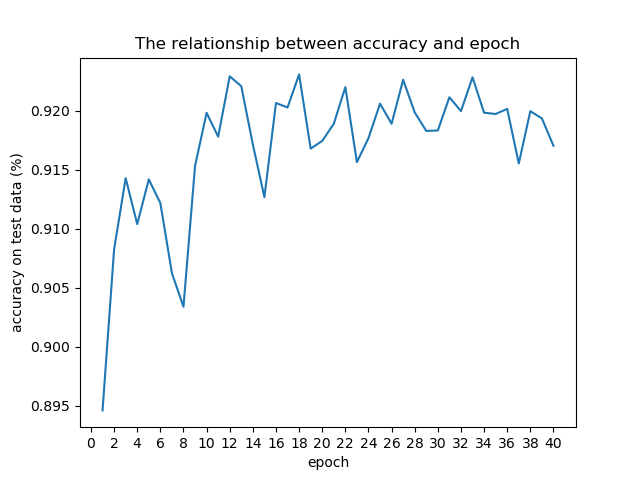
\includegraphics[width=\linewidth]{figuras/epoch_accuracy.png}
\caption{UNet+++ training accuracy-epoch curve}
\label{fig:unetpppCurve}
\end{figure}

The curve shows that as the epoch value increase, the accuracy first increase rapidly and than decrease slowly, 
which means that when epoch is too large, it becomes overfitting.
The best accuracy is 0.923, with the epoch value 18
